% 在 Linux 上编译 C/C++ 程序
% linux|c++|gcc|g++

本文介绍如何使用 Linux 控制行用 g++ 编译器编译一个 C++ 的 hello world 程序. 阅读本文不需要任何基础(包括 C++ 和 Linux).

如何安装 Linux 控制行? 你可以直接在电脑上安装一个 Linux 系统, 也可以在 Win10 下使用 WSL(已经安装 win10 系统的话建议使用后者), 如果是 win7 系统, 可以安装一个 MinGW. 安装方法请自行搜索. 本文以 Ubuntu 系统为例(Linux 有不同的版本, Ubuntu 是广泛使用的一个).

\subsection{在控制行安装 g++}
打开控制行后, 要检查是否安装了 g++, 输入以下命令并按回车.
\begin{lstlisting}[language=bash]
g++ --version
\end{lstlisting}
这个命令由两部分组成, 第一部分是 \lstinline|g++|, 即在控制行中调用 \lstinline|g++| 这个程序. 第二部分是 g++ 程序的 \lstinline|--version| 选项, 即查看已安装 g++ 的版本. 如果系统上没有安装 g++, 控制行(Terminal)会返回类似这样的提示
\begin{lstlisting}[language=bash]
Command 'g++' not found, but can be installed with:
sudo apt install g++
\end{lstlisting}
要安装 g++, 只需要在 terminal 输入两个命令
\begin{lstlisting}[language=bash]
sudo apt update
sudo apt install g++
\end{lstlisting}
\lstinline|sudo| 是 super user do, 即获取操作系统的 root 权限, root 权限是 Linux 系统的最高权限. 控制行中的一些命令(如安装卸载软件)一般需要 root 权限, 所以需要在前面加 sudo (如果你已经以 root 的身份登录 Linux 则不需要).

\lstinline|apt| (也可以用 \lstinline|apt-get|) 是 Ubuntu 系统中用来管理程序的命令(安装,卸载,更新等). 注意系统一般要链接网络才能使用 apt 安装程序. 在安装任何程序之前, 建议新更新一下 apt 的数据库(第一行).

\lstinline|update| 是 \lstinline|apt| 的一个参数(argument), 就跟 g++ 的 \lstinline|--version| 参数一样. Linux 中程序的许多参数以 \lstinline|--| 或者 \lstinline|-| 开头.

\lstinline|install| 是 \lstinline|apt| 程序的另一个参数. \lstinline|g++| 是 \lstinline|install| 的参数, 即要安装的软件名.

运行后可以按提示安装 g++, 过程中可能需要输入 Linux 的用户密码, 以及确认是否安装(输入 \lstinline|Y| 然后按回车)
\begin{lstlisting}[language=bash]
After this operation, 155 MB of additional disk space will be used.
Do you want to continue? [Y/n] Y
\end{lstlisting}

安装完以后, 再次查看 g++ 的 version, 得到
\begin{lstlisting}[language=bash]
g++ (Ubuntu 7.4.0-1ubuntu1~18.04.1) 7.4.0
Copyright (C) 2017 Free Software Foundation, Inc.
This is free software; see the source for copying conditions.  There is NO
warranty; not even for MERCHANTABILITY or FITNESS FOR A PARTICULAR PURPOSE.
\end{lstlisting}
可以看到我们安装的版本是 7.4.0.


\subsection{创建第一个 C++ 程序}
打开一个文本编辑器, 创建一个新文本文档, 命名为 hello.cpp, 输入如下 C++ 代码并保存.
\begin{lstlisting}[language=bash]
// print hello world
#include <iostream>

int main()
{
    std::cout << "hello world!" << std::endl;
}
\end{lstlisting}
在编译之前, 我们首先要介绍 working directory. 控制行一般会在输入的每一行命令之前显示当前的路径(directory)如\autoref{linCpp_fig1}.
\begin{figure}[ht]
\centering
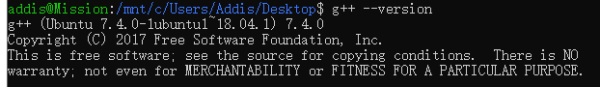
\includegraphics[width=14cm]{./figures/linCpp_1.png}
\caption{蓝色的路径就是当前路径} \label{linCpp_fig1}
\end{figure}

这个目录一般是打开控制行的目录(例如 Ubuntu 中在某个文件夹中右键打开控制行, 或者 win10 中按 shift + 右键). 我们假设刚才创建的 cpp 文件就保存在这个目录下.

现在我们来用 g++ 编译这个程序, 控制行输入
\begin{lstlisting}[language=bash]
g++ hello.cpp
\end{lstlisting}
如果编译成功, 将会在同一文件夹中生成 a.out 可执行文件, 相当于 windows 中的 exe 文件. 要运行该文件, 使用(\lstinline|./| 表示当前的 working directory)
\begin{lstlisting}[language=bash]
./a.out
\end{lstlisting}
运行后可以看到程序在控制行输出了 \lstinline|hello world!|.

这样, 我们就成功在 Linux 中运行了第一个 C++ 程序.
